%% NetMob DC 2026 -- complete document (confidential), submission #32166
%% Extends the accepted 2-page abstract of the same title.
%% Compile on Overleaf with the official NetMob 2026 / opticajnl template.
%% All figures live in ./figures/ .

\documentclass[9pt,twocolumn,twoside]{opticajnl}
\journal{opticajournal}

\setboolean{shortarticle}{false}

\usepackage{lineno}
\usepackage{booktabs}

\title{Finite-size--corrected synchronization in a city-scale bus network:
crossover, not criticality}

\author[1,*]{Po-Hsun, Lai}

\affil[1]{Physics, National Taiwan University, Taipei, Taiwan}

\affil[*]{b11202025@ntu.edu.tw}

\setboolean{displaycopyright}{false}

\graphicspath{{../Figure/}{./}}

\begin{abstract}
Bus bunching is widely read as phase synchronization of coupled oscillators, with sustained
clustering emerging once passenger demand exceeds a threshold. Testing that picture on real
networks requires a synchronization observable that is comparable across time and place --- and
the natural one is not. On 13.8M GPS fixes and 6.8M boardings from the NetMob26 Niter\'oi
dataset, the raw Kuramoto order parameter is severely confounded by the number of buses in a
cell: small fleets read as synchronized for purely statistical reasons. Correcting against a
same-$N$ random-phase null overturns the apparent weekend effect and recasts the demand
dependence as a smooth crossover rather than a sharp critical transition. Downstream headway
amplification is more strongly associated with inherited upstream irregularity than with
realized load, and the co-synchronization of lines on a shared trunk is largely consistent with
shared road-state exposure once segment speed is controlled. This document extends the accepted
abstract with the evidence needed to judge those claims. We put the finite-size correction on an
exact footing using Kluyver's solution of Pearson's random walk, showing that the Rayleigh
asymptotic in common use is biased by 1.5--2.5\% exactly where transit data live; we compare
five normalisations, including the analytically unbiased pairwise phase consistency imported
from neurophysiology, and four null models; we add a finite-size scaling collapse with a
permutation control; and we derive the Newell--Potts prediction that bunching has no threshold
in load, which makes ``crossover, not criticality'' a theoretical expectation rather than a null
result. Two refinements survive that scrutiny and sharpen the original claims. The weekend
result is better described as an abolition than a reversal: matched on $N$, the contrast is
statistically indistinguishable from zero in all 25 estimator-by-null combinations, so the
marginal and conditional comparisons are different estimands. And half of all active bus-hours
sit within 10\% of a route terminal, where buses are clustered by construction; trimming 2\% from
each route end turns the mean corrected order parameter from $+0.15$ to $-0.12$, and the demand
association --- present on the whole route --- is absent within every route zone taken separately.
What reads as collective synchronization in raw transit data is, here, a mixture of finite-size
bias, route-position structure, operational dispatch irregularity, and common road-state shocks.
Finite-size null correction is a prerequisite for interpreting field synchronization observables
as collective dynamics; on any system with boundaries, so is knowing where the oscillators sit.
\end{abstract}

\begin{document}

\maketitle

\section{Introduction}

This is, before it is a study of buses, a study of a measurement problem: what it takes for a
synchronization observable measured in the field to mean the same thing twice. The transit
network is where we can test that, because it is one of the few settings in which the ensemble
size, the load, and the geometry are all observed directly.

A bus that falls behind schedule meets more waiting passengers, dwells longer, and falls
further behind, until the following bus catches it: the headways collapse and buses bunch.
Newell and Potts framed this instability in 1964 \cite{newell64}, and a complex-systems reading
treats each line as a ring of coupled self-oscillators whose phases lock under load, in analogy
with the Kuramoto transition \cite{saw19,strogatz00,kuramoto75}. That analogy predicts a
demand-driven onset of collective synchronization. It has been examined almost entirely in
simulation or on single shuttle loops; a city-scale, multi-line test with fused vehicle
telemetry and passenger demand has been missing, largely for want of such data
\cite{schlapfer21}. The NetMob26 dataset \cite{netmob26} supplies it for Niter\'oi, Brazil.

The central methodological point of this work is that the observable comes first. Before one can
ask whether a transit network shows a demand-driven synchronization transition, one needs a
synchronization measure that means the same thing in a cell with three active buses as in a cell
with twenty. The Kuramoto order parameter does not. For $N$ uniformly random phases
$\mathbb{E}[r_1]\approx 0.886/\sqrt{N}$, so any quantity that covaries with fleet size ---
weekends, off-peak hours, low-demand lines --- inherits a spurious synchronization signal. The
correction we apply, and the discipline of reporting every value with its $N$, is the
prerequisite for everything that follows.

\paragraph{What this document adds.} The accepted abstract reported three results from a
four-phase analysis. This complete document retains all of them and supplies the evidence and
robustness checks that two pages could not carry. Specifically:
\begin{enumerate}\itemsep1pt
\item \textbf{An exact foundation for the correction} (Sec.~\ref{sec:null}). The null
      distribution of $r_1$ is Kluyver's solution of Pearson's random walk; we validate our
      Monte Carlo null against it as a unit test, and quantify how badly the Rayleigh asymptotic
      quoted throughout this literature fails at the fleet sizes transit data actually contain.
\item \textbf{A comparison against alternative normalisations} (Sec.~\ref{sec:estimators}),
      including the pairwise phase consistency of Vinck et al.\ \cite{vinck10}, which solves the
      same problem in neurophysiology, is analytically unbiased, and needs no simulation.
\item \textbf{Null-model sensitivity} (Sec.~\ref{sec:nullmodels}): four nulls spanning a nested
      hierarchy of preserved structure, so the dependence on the random-phase assumption is
      measured rather than acknowledged.
\item \textbf{A theoretical account} (Sec.~\ref{sec:assump}) of which Kuramoto assumptions a bus
      route violates, with the Newell--Potts growth rate derived, validated numerically, and the
      mean-field critical coupling estimated from the observed distribution of route run times.
\item \textbf{A finite-size scaling collapse with a permutation control}
      (Sec.~\ref{sec:crossover}), which is the statistical-physics test that our pre-registered
      three-part gate was standing in for.
\item \textbf{Two refinements to the original claims} (Sec.~\ref{sec:weekend} and
      Sec.~\ref{sec:position}), reported in full because both change how the results should be
      read: the weekend effect is abolished rather than reversed once conditioned on $N$, and
      the demand association on the whole route is substantially a route-position mixture.
\end{enumerate}
Sections~\ref{sec:data}--\ref{sec:assump} develop the data, observable and theory;
Sec.~\ref{sec:results} gives the results in the order of the accepted abstract;
Sec.~\ref{sec:position} is the route-position robustness check; Secs.~\ref{sec:discussion}
and~\ref{sec:limits} discuss generality and limitations. All analysis code, with fixed seeds and
21 unit tests, is described in Appendix~\ref{app:repro}.

\section{Data, analysis unit, and preprocessing}\label{sec:data}

\subsection{Sources and coverage}

We use 19 days of telemetry (11--31 March 2026; 13{,}850{,}467 GPS fixes from 527 vehicles at
15--30\,s spacing) and the full ticketing feed (6{,}790{,}681 boardings), together with the
GTFS schedule feeds for the two operators, the official bus-stop inventory, and the hourly
meteorological series.

\subsection{The identification scope is fixed by the data}

The telemetry and ticketing feeds carry no common vehicle key. The mobility \texttt{id} field and
the ticketing \texttt{vehicle\_number} field have 527 and 556 distinct values respectively and
\emph{zero} overlap. This is not a normalisation failure on our part: both fields are purely
numeric, and their ranges are \emph{disjoint} --- $52{,}243$--$136{,}462$ for telemetry against
$2{,}001$--$24{,}142$ for ticketing --- so no formatting repair or approximate match could join
them. The dataset documentation states what they are: \texttt{id} is a ``hardware/transponder
ID'', whereas \texttt{vehicle\_number} is the operator's ``bus ID''. They are different
identifier systems by definition, the release contains no crosswalk between them, and the GTFS
feeds carry no vehicle table.

The two feeds do describe the same system. Restricted to the telemetry period, ticketing records
550 distinct vehicles against the telemetry's 527; all six operators present in the ticketing
\texttt{company\_number} field have telemetry coverage of 50--100\% of their routes; and 46
route labels appear in both. We therefore treat the two identifier spaces as two numberings of
one fleet, while noting that the release does not document this and no vehicle-level
correspondence can be recovered from it.

The only usable link is the route label, and even that needs care: the same line appears as
\texttt{24} and \texttt{24.0}, as \texttt{3} and \texttt{03}, and as \texttt{62B} and
\texttt{62} across the two feeds, so demand is joined on a normalised line code with an explicit
alias table rather than on the raw strings.

This is not a nuisance to be worked around; it fixes the identification scope of the entire
study. Passenger exposure can only be defined at the
\textit{line--direction--hour} level, and every demand-related quantity below is cell-level
rather than vehicle-level. We treat that as the analysis unit by design, and we write
$\lambda = \text{boardings}/N$ for realized load per active bus, which is not exogenous
passenger demand: $N$ is itself an operational response to demand and conditions, and
headway-based control changes the effective coupling directly \cite{daganzo09}.

One consequence should be stated at the outset rather than in a closing caveat, because it
governs how one result below must be read. Since boardings cannot be attributed to individual
vehicles, no test in this document can resolve a vehicle-level dwell-time mechanism. The
dwell-mediation analysis of Sec.~\ref{sec:mechanisms} is therefore \emph{inconclusive} about
that channel rather than evidence against it, and we do not read it as ruling the mechanism out.

\subsection{Map matching and exclusions}

For each of 20 high-ridership lines we project GPS onto the route polyline
(\texttt{line\_routes.json}, with GTFS \texttt{shapes.txt} as fallback) and reduce position to
arc length $s$. Trajectories are resampled to a 30\,s grid, with interpolation suppressed across
gaps longer than 3 minutes and across apparent jumps exceeding 50\% of route length.
Terminal-layover bus-hours (at least 10 minutes, at least 75\% of samples within 5\% of an
endpoint, arc span $\le 150$\,m) are excluded, as are sparsely sampled bus-hours and those with
high matching residual; 3{,}920, 11{,}326 and 948 bus-hours respectively. This leaves
69{,}466 active bus-hours in 10{,}135 analysis-eligible cells.

Matching quality is high and, importantly for Sec.~\ref{sec:position}, uniform along the route:
median residuals are 4.13\,m in the route interior, 3.89\,m near terminals and 4.24\,m at
terminals. Whatever the terminal concentration documented later is, it is not a projection
artefact.

\subsection{Two phase definitions}\label{sec:phase}

The standard construction assigns $\varphi_{\rm arc} = 2\pi s / L$ per direction, so the buses on
a \textit{(line, direction, hour)} cell become oscillators on a ring. This violates the
assumption the Kuramoto analogy rests on, that a free-running oscillator advances its phase at a
constant rate: a bus does not cover arc length at a constant rate, so arc-length phase piles up
wherever the bus is slow. We therefore also construct a time-parametrised phase
\begin{equation}
\varphi_{\rm time} = 2\pi\, T(s)/T_{\rm cycle},
\label{eq:timephase}
\end{equation}
with $T(s)$ the median cumulative travel time to arc position $s$, estimated from the times at
which vehicles cross 11 fixed cross-sections of each route. Individual vehicle-days are first
separated into trips by detecting the arc-length reset at each terminal, so that successive
round trips are not pooled. Profiles are recovered for all 40 line-directions, covering 100\% of
active bus-hours.

Route speed is markedly non-uniform. For line 30 direction 0, the first half of the route by
distance accounts for 60\% of the travel time; across all line-directions the median maximum
departure of $T(s)/T_{\rm cycle}$ from $s/L$ is 0.086, reaching 0.60. Under
$\varphi_{\rm time}$ a free-running bus advances phase at a constant rate by construction, so an
evenly spaced timetable maps to an even spread of phase --- which is what the uniform null
assumes. We report both definitions throughout; where they differ, we say so.

\section{The synchronization observable}\label{sec:obs}

\subsection{Order parameter}

For a cell of $N$ buses we compute the Kuramoto--Daido order parameters
\begin{equation}
r_m = \Big| \tfrac{1}{N}\sum_{j=1}^{N} e^{im\varphi_j} \Big|,
\label{eq:rm}
\end{equation}
with $r_1$ near $0$ for evenly spread buses (the splay state) and near $1$ when they bunch.
Higher harmonics $r_2, r_3$ \cite{daido90} detect two- and three-cluster configurations that
$r_1$ misses entirely; we use them in Sec.~\ref{sec:crossover} as a shape diagnostic.

It is worth recording what $r_1$ measures. Writing $\varphi_j = 2\pi j/N + \epsilon_j$ for small
deviations about the splay state,
\begin{equation}
r_1 \;\approx\; \Big|\tfrac{1}{N}\textstyle\sum_j \epsilon_j\, e^{i 2\pi j/N}\Big| ,
\label{eq:mode1}
\end{equation}
so $r_1$ is the amplitude of the \emph{first Fourier mode} of the headway deviation field --- one
specific mode, not a general measure of irregularity. This is what connects the order parameter
to the headway-CV language of the transit literature, and it is what makes the quantitative
prediction of Sec.~\ref{sec:assump} possible.

\subsection{Why the bias arises, and the exact null}\label{sec:null}

Under $N$ i.i.d.\ uniform phases, $N r_1$ is the endpoint of an $N$-step unit random walk in the
plane. Its distribution is Pearson's random-walk problem, solved by Kluyver in 1905
\cite{kluyver05}:
\begin{equation}
\Pr(r_1 \le x) \;=\; N x \int_0^{\infty} J_1(Nxt)\, J_0(t)^{N}\, dt ,
\label{eq:kluyver}
\end{equation}
from which
\begin{equation}
\mathbb{E}[r_1^2] = \frac{1}{N} \ \text{exactly for every } N, \qquad
\mathbb{E}[r_1]\big|_{N=2} = \frac{2}{\pi} .
\label{eq:moments}
\end{equation}
The familiar $0.886/\sqrt{N}$ is only the large-$N$ (Rayleigh) limit of the mean.

The distinction is not academic here. The median cell in this dataset has $N = 6$ and the lower
quartile $N = 4$, so the asymptotic expression is being applied well outside its range of
validity. We draw $20{,}000$ random-phase samples at each observed $N$ and validate the resulting
null against Eq.~\eqref{eq:kluyver}: agreement is within $0.01$ in CDF for $N = 2\ldots8$ at
$x = 0.2, 0.4, 0.6, 0.8$, and within Monte Carlo error ($<0.15\%$) in the mean, while the
Rayleigh asymptotic is biased by $1.5$--$2.5\%$ over $N = 2\ldots5$
(Fig.~\ref{fig:obs}b). The validations run as unit tests shipped with the code.

We then report the finite-size--corrected synchronization
\begin{equation}
r_{\mathrm{exc}} = \frac{r_1 - \mathbb{E}_{\mathrm{null}}[r_1|N]}{1 - \mathbb{E}_{\mathrm{null}}[r_1|N]},
\qquad
z = \frac{r_1 - \mathbb{E}_{\mathrm{null}}[r_1|N]}{\mathrm{sd}_{\mathrm{null}}[r_1|N]} ,
\label{eq:rexc}
\end{equation}
which measure how far a cell sits above its same-$N$ random baseline.

\begin{figure*}[t]
\centering
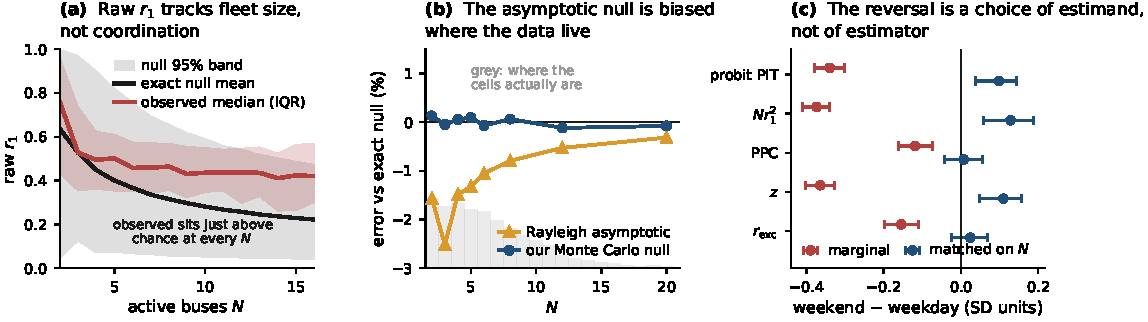
\includegraphics[width=\textwidth]{f1_observable.pdf}
\caption{The observable, its exact null, and what correcting it does and does not buy.
(a) Observed $r_1$ (median and IQR) against fleet size, with the exact same-$N$ null and its
95\% band. Small cells report high $r_1$ for purely statistical reasons.
(b) Error of each null relative to the exact Kluyver solution, with the distribution of observed
$N$ shaded behind. The Rayleigh asymptotic in common use is biased by 1.5--2.5\% exactly where
the data live; our Monte Carlo null is unbiased to within its sampling error.
(c) Weekend$-$weekday contrast for five estimators in units of each estimator's own cell-level
standard deviation, computed marginally and matched on $N$. Every estimator shows the same
pattern; the disagreement is between estimands, not estimators (Sec.~\ref{sec:weekend}).}
\label{fig:obs}
\end{figure*}

\subsection{Five normalisations}\label{sec:estimators}

Given a null, there is more than one way to correct, and the choice is not innocuous. Alongside
$r_{\rm exc}$ and $z$ we compute
\begin{equation}
{\rm PPC} = \frac{N r_1^2 - 1}{N-1}, \qquad
Z_R = N r_1^2 ,
\label{eq:ppc}
\end{equation}
and the probability integral transform $\Phi^{-1}(F_{\rm null}(r_1|N))$, which is exactly
standard normal under the null at every $N$ and is therefore the strictest available control.

PPC deserves emphasis because it is not our construction. It is the pairwise phase consistency of
Vinck et al.\ \cite{vinck10}, developed in neurophysiology for exactly this problem --- the
phase-locking value and spectral coherence are positively biased at finite sample size --- and it
equals the mean of $\cos(\varphi_j - \varphi_k)$ over distinct pairs. Its population parameter is
the squared population resultant, and it is \emph{analytically} unbiased for that quantity under
i.i.d.\ sampling, at any true value, with no Monte Carlo null required. We verified the algebraic
identity between Eq.~\eqref{eq:ppc} and the pairwise form both symbolically and against the
reference implementation in FieldTrip. That a field with a twenty-year head start on this
problem converged on a debiased second-moment estimator rather than a rescaled first-moment one
is informative, and Table~\ref{tab:gradient} shows why.

\subsection{Which normalisation, and by what criterion}\label{sec:criterion}

Comparing normalisations requires stating what a good one has to do. We use five criteria, in
descending order of importance for field data:

\begin{enumerate}\itemsep1pt
\item \textbf{Null-unbiasedness.} Expectation zero under the same-$N$ null, at every $N$.
      All five satisfy this by construction; it is necessary but far too weak.
\item \textbf{Unbiasedness under the alternative.} The estimator should be unbiased for a
      population quantity at any true value, not only at zero. This is where the five separate:
      only PPC has it analytically, because $\mathbb{E}[r_1^2] = \rho^2 + (1-\rho^2)/N$ under
      i.i.d.\ sampling makes Eq.~\eqref{eq:ppc} unbiased for $\rho^2$ for every $\rho$.
      $r_{\rm exc}$ rescales a first moment whose bias is only removed at $\rho = 0$.
\item \textbf{Residual $N$-dependence.} The empirical consequence of criterion 2, measured in
      Table~\ref{tab:gradient}. Any surviving gradient means group comparisons remain confounded
      whenever fleet size differs between groups --- which is the situation this paper is about.
\item \textbf{Independence from the null model.} A closed-form estimator cannot inherit
      misspecification of the null. PPC and $Z_R$ are closed form; $r_{\rm exc}$, $z$ and the
      PIT are not, and Table~\ref{tab:gradient} shows how much the latter three move when the
      null changes.
\item \textbf{Interpretability on a bounded scale.} $r_{\rm exc}$ is $0$ at chance and $1$ at
      perfect bunching, which is why we retain it for reporting; $Z_R$ is on an unbounded scale
      that grows with $N$ and is unusable for cross-cell comparison.
\end{enumerate}

\noindent
No single estimator wins on all five, and we do not claim that $r_{\rm exc}$ --- the choice in
the accepted abstract --- is optimal. On criteria 2--4 PPC is strictly better, and we recommend
it as the default for future work of this kind. What Eq.~\eqref{eq:rexc} buys is criterion 5,
and the results below are reported under both so that nothing rests on the choice. The
substantive finding of Sec.~\ref{sec:weekend} is that all five agree on the direction of every
contrast once the estimand is fixed, which is the strongest evidence we can offer that the
conclusions are not an artefact of the normalisation.

\subsection{Four null models, and what they assume}\label{sec:nullmodels}

The uniform null encodes ``perfect service $=$ buses evenly spread in arc length'', which is not
what perfect service means: a route with a congested stretch accumulates buses there even at
perfectly regular headways. We therefore also build a \textbf{speed-weighted} null, with phases
drawn uniform in travel time and mapped back to arc-length phase (equivalently, arc-length
density $\propto 1/v(s)$), which is the null implied by evenly spaced headways in time; an
\textbf{occupancy} null, resampling from the observed marginal distribution of arc-length
position, which absorbs route geometry wholesale; and a per-route \textbf{permutation} null.
These form a nested hierarchy of preserved structure. Every headline result below is recomputed
under each.

\paragraph{What the random-phase null assumes.} Three assumptions are embedded in
Eq.~\eqref{eq:kluyver}, and it is worth separating them because they fail differently.

\emph{(i) Uniformity.} That ideal service puts buses uniformly in the phase coordinate. Under
$\varphi_{\rm arc}$ this is false whenever route speed varies, since a bus dwells longer in
phase where it moves slower; the speed-weighted null and the time-parametrised phase of
Sec.~\ref{sec:phase} are two views of the same repair. It is false for a second and larger
reason on an open route, where vehicles accumulate at the terminals: that failure is not
repaired by either device, and Sec.~\ref{sec:position} is the consequence. This is the
assumption that matters most in these data.

\emph{(ii) Exchangeability.} That the $N$ phases in a cell are i.i.d.\ draws. The
unidirectional coupling of Sec.~\ref{sec:assump} formally violates this: bus $n$'s position
depends on bus $n-1$'s. The null is therefore a null of \emph{no coordination given the
occupancy}, not a generative model of the fleet, and $r_{\rm exc}$ should be read as an excess
over chance rather than as an estimate of a coupling strength. The per-route permutation null
is the least committal alternative we have, because it preserves each route's own occupancy and
destroys only within-hour simultaneity.

\emph{(iii) Ancillarity of $N$.} That conditioning on $N$ does not itself condition on the
quantity of interest. This fails when $N$ mediates the comparison being made, which is exactly
the weekend case: fewer buses is part of what a weekend \emph{is}. That is why
Sec.~\ref{sec:weekend} reports marginal and conditional contrasts as separate estimands rather
than choosing between them.

None of the three is fully satisfied here. Our response is to measure the sensitivity rather
than argue the assumptions away: Table~\ref{tab:gradient} reports how much each estimator moves
across nulls, and the direction of every headline result is reported under all four.

\section{What the Kuramoto analogy assumes}\label{sec:assump}

The mean-field Kuramoto model,
$\dot\varphi_i = \omega_i + (K/N)\sum_j \sin(\varphi_j - \varphi_i)$, is the reference point for
reading bunching as synchronization. A bus network violates most of its assumptions, and the
violations are not incidental: they change what should be expected, and they are the reason we
regard ``crossover, not criticality'' as a confirmation rather than a null result.

\textbf{(K1) Constant free-running phase velocity.} Violated by $\varphi_{\rm arc}$, as
discussed in Sec.~\ref{sec:phase}; repaired by $\varphi_{\rm time}$.

\textbf{(K2) All-to-all coupling.} Buses interact with the vehicle ahead, and the interaction is
\emph{unidirectional}: a bus is delayed by passengers its leader failed to collect, while the
leader is unaffected by what follows. Chew, Saw and Pang \cite{chew19} studied precisely this
local unidirectional variant and found that stable anti-bunched states require at least five
oscillators. Our median cell has $N = 6$ and our lower quartile $N = 4$: this system operates at
the theoretical stability boundary.

\textbf{(K3) Attractive coupling toward a mean phase.} There is no restoring force toward a
common phase; the splay state is an unstable fixed point and the bunched state is absorbing
\cite{gershenson09}. The dynamics are a one-way drift, not a symmetry-breaking transition.

\textbf{(K4) A closed ring.} Bus routes are open, and terminals reset phase every cycle. A ring
cut once per revolution cannot accumulate the long-range order a critical state requires ---
and, as Sec.~\ref{sec:position} shows, the terminals do considerably more damage than that.

\textbf{(K5) A fixed distribution of natural frequencies.} We estimate $g(\omega)$ directly from
30{,}896 near-complete route traversals. The dispersion is large: the median coefficient of
variation of run time is $0.235$, giving $\sigma_\omega = 0.033$\,rad/min against a mean
$\omega$ of $0.137$\,rad/min. The implied mean-field threshold $K_c = 2/\pi g(0)$ has median
$0.055$\,rad/min, i.e.\ $0.38\,\omega$: entraining this ensemble in the mean-field sense would
require a coupling comparable to the orbital frequency itself (Fig.~\ref{fig:theory}c).

\textbf{(K6) The thermodynamic limit.} With median $N = 6$, finite-size effects are not a
correction here; they are the leading term.

\subsection{What the appropriate model predicts}

The right reference model is not Kuramoto but Newell--Potts. With dwell time proportional to
passengers accumulated since the previous bus, headways obey
\begin{equation}
h_{n,j+1} = (1+k)\,h_{n,j} - k\,h_{n-1,j},
\label{eq:np}
\end{equation}
for bus $n$ at stop $j$, where $k$ is the ratio of passenger arrival rate to boarding rate.
Substituting $h_{n,j} = A^j e^{i\theta n}$ gives
\begin{equation}
A(\theta) = (1+k) - k e^{-i\theta}, \quad
|A|^2 = (1+k)^2 - 2k(1+k)\cos\theta + k^2 .
\label{eq:growth}
\end{equation}
Three consequences matter. First, $|A(0)| = 1$ exactly: a uniform timetable shift is neutral, as
it must be. Second, and centrally,
\begin{equation}
|A(\theta)| > 1 \quad \text{for every } \theta \neq 0 \text{ and every } k > 0 :
\end{equation}
\emph{there is no threshold in $k$}. Bunching is an unconditional instability whose \emph{rate}
increases smoothly with load. A smooth crossover is therefore what the correct model predicts,
and the absence of a sharp transition in Sec.~\ref{sec:crossover} is a confirmation of theory
rather than a weakened version of a positive finding. Third, by Eq.~\eqref{eq:mode1} the mode
that $r_1$ measures is $\theta = 2\pi/N$, so the model predicts the growth of the order
parameter itself,
\begin{equation}
\frac{d \ln r_1}{d\,\text{stop}} = \ln|A(2\pi/N)| \;\xrightarrow[\text{large }N]{}\;
\frac{2\pi^2 k(1+k)}{N^2},
\label{eq:mode1growth}
\end{equation}
while headway CV, which loads on all modes, is dominated by $\theta = \pi$ where
$|A| = 1+2k$. We verified Eq.~\eqref{eq:mode1growth} against direct simulation of
Eq.~\eqref{eq:np} on a ring, recovering the predicted rate to within $0.1\%$ across
$N \in \{4,8,16\}$ and $k \in \{0.05, 0.2, 0.5\}$. Because $k$ and $N$ are both measurable, this
is a prediction with nothing left to fit; Sec.~\ref{sec:mechanisms} tests it.

\begin{figure*}[t]
\centering
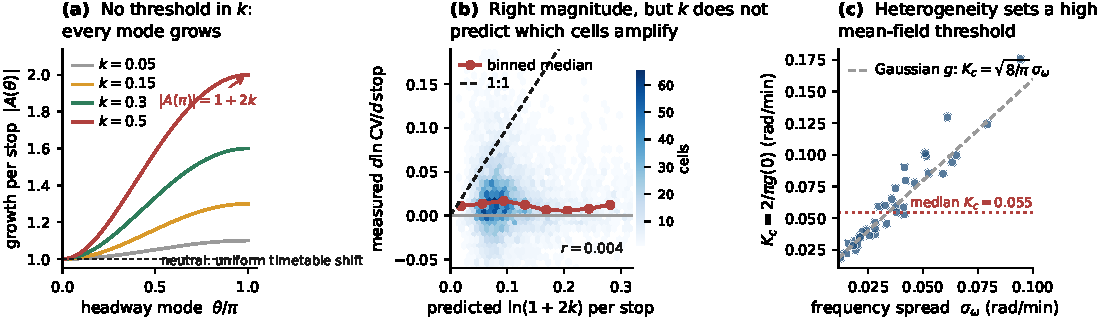
\includegraphics[width=\textwidth]{f3_theory.pdf}
\caption{Theory with independently measured parameters.
(a) Newell--Potts per-stop growth factor $|A(\theta)|$ from Eq.~\eqref{eq:growth}. Every mode
with $\theta \neq 0$ grows for every $k>0$: there is no threshold, so a smooth load dependence is
the prediction, not a surprise.
(b) Measured against predicted per-stop growth of headway irregularity across 6105 cells, shown
as a hexbin with binned medians. The magnitude is of the predicted order, but $k$ does not
predict which cells amplify ($r = 0.004$, $p = 0.73$).
(c) Mean-field critical coupling $K_c = 2/\pi g(0)$ against the natural-frequency spread, one
point per line-direction, from 30{,}896 observed route traversals.}
\label{fig:theory}
\end{figure*}

\section{Results}\label{sec:results}

\subsection{Result 1 --- finite-size correction and the weekend effect}\label{sec:weekend}

In the raw signal, weekends look \emph{more} synchronized than weekdays
(weekend$-$weekday $r_1 = +0.047$, 95\% CI $[0.039, 0.056]$) despite running far fewer buses
($\bar N = 4.47$ against $7.99$). This is exactly the regime where $r_1$ is least trustworthy,
and correcting against the same-$N$ null overturns the marginal comparison:
$r_{\mathrm{exc}} = -0.066$ $([-0.084,-0.047])$ and $z = -0.440$ $([-0.485,-0.396])$.
Corrected synchronization is lower on weekends. This remains the clearest empirical
demonstration in these data that raw Kuramoto observables cannot be compared across cells of
different $N$.

The extended analysis refines how the change of sign should be described, and we report the
refinement because it matters for interpretation. Matching cells exactly on $N$ and weighting
strata by cell count, the contrast becomes $+0.010$ $([-0.010, +0.029])$ --- indistinguishable
from zero. The reason is that the corrections remove the null's first moment but not the
estimator's residual $N$-dependence under the alternative: mean $r_{\rm exc}$ rises from $0.10$
at $N=2$ to $0.28$ at $N=15$. Since weekends have systematically smaller fleets, the marginal
contrast still runs partly through $N$.

Table~\ref{tab:contrasts} shows this is not an artefact of one estimator. Across five estimators
and five phase-by-null specifications, 23 of 25 marginal contrasts are negative and \emph{all
25} conditional contrasts are positive; two analytically unbiased estimators behave exactly like
the Monte Carlo ones. The accurate statement has three parts, all true simultaneously:
\begin{enumerate}\itemsep0pt
\item the raw weekend difference is almost entirely fleet-size composition ($+0.047 \to +0.014$
      once matched on $N$) --- a \emph{stronger} demonstration of this paper's core point than
      the sign change alone;
\item the corrected \emph{total} effect is negative, because $N$ is itself a mediator: weekends
      run fewer buses, and fewer buses genuinely means less clustering;
\item conditional on $N$, there is no weekend effect.
\end{enumerate}
Marginal and conditional contrasts are different estimands, and reporting only one of them is
what creates the appearance of a contradiction.

\begin{table}[t]
\centering
\caption{\bf Weekend$-$weekday contrast by estimator, arc phase, uniform null$^{a}$}
\small
\setlength{\tabcolsep}{3.2pt}
\begin{tabular}{lcc}
\toprule
Estimator & Marginal & Matched on $N$ \\
\midrule
$r_1$ (raw)          & $+0.047$ & $+0.014\ [+0.002,+0.025]$ \\
$r_{\rm exc}$        & $-0.066\ [-0.084,-0.047]$ & $+0.010\ [-0.010,+0.029]$ \\
$z$                  & $-0.440\ [-0.485,-0.396]$ & $+0.133\ [+0.059,+0.191]$ \\
PPC                  & $-0.042\ [-0.057,-0.026]$ & $+0.003\ [-0.015,+0.019]$ \\
$Z_R = Nr_1^2$       & $-0.562\ [-0.617,-0.511]$ & $+0.193\ [+0.089,+0.282]$ \\
probit PIT           & $-0.381\ [-0.424,-0.338]$ & $+0.111\ [+0.041,+0.162]$ \\
\bottomrule
\end{tabular}
\label{tab:contrasts}

\smallskip
$^{a}$Percentile bootstrap over cells, 2000 draws. Across all five phase-by-null
specifications, 23/25 marginal contrasts are negative and 25/25 conditional contrasts are
positive.
\end{table}

\paragraph{Which estimator to prefer.} Table~\ref{tab:gradient} reports the residual
$N$-dependence each normalisation leaves, as the slope of the estimator mean on $\log N$. PPC
leaves roughly half the gradient of $r_{\rm exc}$ (0.059 against 0.117) and, being closed-form,
is invariant to the null model; we recommend it as the default for future work of this kind,
with $r_{\rm exc}$ retained for continuity. $Z_R$ is unusable for cross-$N$ comparison, as
expected from its explicit $N$ factor. Note also that switching from the uniform to the
occupancy null cuts the residual gradient of $z$ from 1.61 to 0.28 and of the PIT from 1.27 to
0.28: most of the apparent $N$-dependence of those statistics is route occupancy structure. That
is the first indication of what Sec.~\ref{sec:position} pursues.

\begin{table}[t]
\centering
\caption{\bf Residual $N$-dependence after correction (slope per $\log N$)$^{a}$}
\small
\setlength{\tabcolsep}{3.2pt}
\begin{tabular}{lccc}
\toprule
Estimator & Uniform null & Speed null & Occupancy null \\
\midrule
PPC            & $0.059$ & $0.059$ & $0.059$ \\
$r_{\rm exc}$  & $0.117$ & $0.110$ & $0.086$ \\
probit PIT     & $1.273$ & $0.983$ & $0.275$ \\
$z$            & $1.612$ & $1.078$ & $0.281$ \\
$Z_R$          & $2.736$ & $2.736$ & $2.736$ \\
\bottomrule
\end{tabular}
\label{tab:gradient}

\smallskip
$^{a}$Zero would mean the correction fully removes fleet-size dependence. PPC and $Z_R$ are
closed-form and so do not vary with the null.
\end{table}

\subsection{Result 2 --- demand modulates synchronization, without a sharp
transition}\label{sec:crossover}

Corrected synchronization rises with realized load per bus: the standardized random-intercept
coefficient is $0.039$ ($p \approx 3\times10^{-15}$), and fleet size enters with a comparable
coefficient ($0.051$). A piecewise fit is preferred over linear and sigmoid alternatives
($\Delta$AIC $=29.4$ and $86.2$) and places an apparent break at $\lambda \approx 136$
boardings per bus, with a bootstrap median of the same value. Weather is a weak modifier: in
530 matched dry/rain cell pairs the corrected difference is $-0.008$ $([-0.038, +0.024])$.

We treat the break as an observational crossover scale rather than a critical point, because a
pre-registered three-part gate does not support criticality. The \emph{susceptibility} check
asks whether fluctuations in $r_{\mathrm{exc}}$ peak at an interior $\lambda$ --- the signature
of a transition, and one with a theoretical warrant, since Daido showed that the intrinsic
fluctuations of the order parameter diverge as a power law at the onset of entrainment
\cite{daido90}. Within $N$-strata they do not (peak/edge ratios $0.89$--$1.14$). The
\emph{coexistence} check asks whether low- and high-synchronization states co-occur near the
candidate scale; the order-parameter distribution is no more bimodal there than elsewhere
($\Delta\mathrm{BIC} \approx 18$, weaker than off-scale regimes). The \emph{$N$-stability} check
asks whether the apparent scale is more than fleet-size composition; this one passes
($|\mathrm{corr}(\lambda_{\rm peak}, N)| = 0.28$). With one of three signatures met, the honest
reading is a smooth, demand-modulated crossover rather than city-scale criticality --- which, by
Sec.~\ref{sec:assump}, is what Eq.~\eqref{eq:growth} predicts.

\paragraph{A finite-size scaling collapse.} The complete document adds the statistical-physics
test the gate was standing in for. If the demand dependence were critical, $r_{\rm exc}$ against
$\lambda$ should collapse across $N$-strata under
$r = N^{-b}F\big((\lambda-\lambda_c)N^{a}\big)$. Two guards are needed to make this a real test
rather than an optimiser artefact: an unnormalised cost is minimised trivially by driving $b$ to
a boundary, shrinking all values toward zero, and the fit can slide strata into disjoint $x$
ranges where within-bin scatter is zero because each bin holds a single stratum. We normalise
the cost by the range of the collapsed ordinate and require at least three strata per bin. We
then benchmark against a permutation control that shuffles $r_{\rm exc}$ within $N$-strata,
preserving the $N$-gradient while destroying any genuine $\lambda$ dependence. Even in the
mean-field Kuramoto model finite-size scaling is subtle, with anomalous sample-dependent effects
and a correlation-size exponent $\bar\nu = 5/2$ \cite{hong07}, so we treat the fitted exponents
as descriptive and rely on the permutation control.

On the whole route the collapse succeeds: improvement ratio $6.56$ against a null median of
$2.63$, permutation $p < 0.017$ (0 of 60 draws), with $a = -1.75$, $b = -1.02$,
$\lambda_c = 32.5$ (Fig.~\ref{fig:collapse}a,c). Taken alone this is the strongest evidence for
scaling in this system we have found, and stronger than the pre-registered gate suggested. It
does not survive the route-position check of Sec.~\ref{sec:position}, and we return to it there.

\paragraph{What the harmonics say.} Correcting each harmonic against its own same-$N$ null, the
corrected $|Z_m|$ is essentially flat in $m$: $0.156$, $0.150$, $0.167$ for $m = 1,2,3$ under arc
phase, and $0.285$, $0.290$, $0.289$ under time phase (Fig.~\ref{fig:collapse}d). This is
diagnostic of shape. A smooth single-mode density modulation --- the picture implied by a
Kuramoto-like transition, where the phase distribution develops one broad peak --- would give
$r_1 \gg r_2 \gg r_3$. To make the comparison concrete we simulate a single von Mises cluster at
the observed $N$ distribution, tuned so that its \emph{corrected} $|Z_1|$ matches the observed
value, and put it through the identical correction: it falls to $\approx 0$ by $m = 2$. Equal
amplitude across harmonics is instead the signature of \emph{compact clusters}, since a
delta-like clump contributes equally to every harmonic. What the order parameter detects in this
system is discrete tight clumps of vehicles.

The two phase definitions differ substantially --- corrected synchronization roughly doubles
under $\varphi_{\rm time}$ (mean $r_{\rm exc}$ $0.154 \to 0.283$; PPC $0.099 \to 0.209$), with
correlation $0.84$. We had expected the opposite sign of change, reasoning that
time-parametrisation stretches congested stretches and should disperse clustered buses. It does;
but it also \emph{compresses} the long fast stretches that occupy much arc length and little
time, and buses spread across those become clustered in time phase. The endpoint mass rises
accordingly, from 0.255/0.256 in the outer deciles under arc phase to 0.287/0.327 under time
phase --- which is the first quantitative hint of Sec.~\ref{sec:position}.

\begin{figure}[t]
\centering
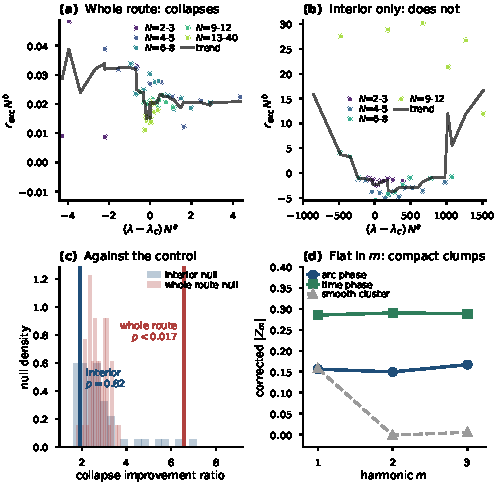
\includegraphics[width=\linewidth]{f4_collapse_harmonics.pdf}
\caption{Scaling and cluster structure. (a) Finite-size scaling collapse of $r_{\rm exc}$
against $\lambda$ across $N$-strata on the whole route. (b) The identical procedure on
interior-only cells. (c) Observed collapse improvement against its permutation control, which
preserves the $N$-gradient but destroys any real $\lambda$ dependence: the whole route beats its
control ($p<0.017$), the interior does not ($p=0.82$). (d) Corrected Daido harmonics. Flatness
in $m$ indicates compact clusters; a single smooth cluster matched at $m=1$ would decay to
$\approx 0$ by $m=2$.}
\label{fig:collapse}
\end{figure}

\subsection{Result 3 --- mechanisms are operational and common-shock
dominated}\label{sec:mechanisms}

We examined three routes by which a genuine oscillator-coupling story might persist.

\paragraph{Downstream amplification.} Headway irregularity grows along the route interior (mean
headway-CV slope $0.12$, $p \approx 2\times10^{-58}$ on the 10--90\% interior), the spatial
fingerprint of the Newell--Potts instability. In a standardized line--direction random-intercept
model (Fig.~\ref{fig:drivers}) this growth is more strongly associated with the irregularity
already inherited upstream ($-0.283$, $[-0.296,-0.270]$) than with contemporaneous realized load
($0.015$, $[0.002,0.027]$) or route topology; the negative sign on the upstream term reflects a
ceiling --- already-irregular hours have less room to grow downstream --- not a stabilizing
effect of irregularity.

The complete document adds the quantitative test this invites. We measure the Newell--Potts load
parameter directly as $k = (\text{mean dwell per stop})/(\text{mean headway})$, avoiding any
assumed boarding rate; its median is $0.048$ (5th--95th percentile $0.023$--$0.173$), placing
this system deep in the low-load regime. Sixty-nine percent of cells show positive growth of
$\ln$ headway CV across the interior, with median rate $0.0129$ per stop, against a
fastest-mode prediction $\ln(1+2k)$ of $0.092$ and a mode-1 prediction $\ln|A(2\pi/N)|$ of
$0.016$. The observed amplification is thus of the order the model predicts and far below the
antiphase-mode ceiling. But the cross-sectional test is negative: across 6{,}105 cells the
correlation between measured and predicted per-stop growth is $r = 0.004$ ($p = 0.73$), so $k$
does not predict \emph{which} cells amplify (Fig.~\ref{fig:theory}b). Amplification is present,
of roughly the right magnitude, and not modulated by load at the cell level --- consistent with
the coefficient ranking above.

\paragraph{Dwell mediation.} The classic $\lambda \to$ dwell-time variability $\to$ bunching
channel is not established in these data: the indirect effect is $\approx 0.0001$
($[-0.0002, +0.0004]$), a mediated proportion of $0.2\%$, over 10{,}082 cell-hours with
1{,}875{,}802 GPS-derived dwell events. As flagged in Sec.~\ref{sec:data}, boardings are not
linked to individual vehicles and GPS-derived dwell is noisy, so this is an
\emph{inconclusive} test of the mechanism, not evidence against it.

\paragraph{Shared corridors.} Lines on a common trunk are more co-synchronized on the shared
segment than off it: across 176 within-pair comparisons the shared-minus-off-trunk gap is
$+0.055$ (sign-flip permutation $p < 0.001$; paired $t$ $p = 1.6\times10^{-4}$), with mean shared
correlation $0.051$ against $-0.005$ off-trunk. Controlling for the shared-segment mean bus speed
--- the common road state --- over 156 pairs with sufficient overlap, the gap falls to $0.018$
$([-0.015, 0.054])$, retaining about a third and now spanning zero. Lead--lag and
transfer-entropy tests show no propagation: only 5.8\% of pairs have a significant non-zero-lag
peak, and the signed directional asymmetry is $0.001$ with permutation $p = 0.87$
(Fig.~\ref{fig:corridor}). The gate verdict is \emph{largely common-shock}: the
co-synchronization is largely consistent with shared road-state exposure, and a residual
inter-line coupling is not established --- though speed control may also absorb part of a
genuine coupling channel, and we do not claim otherwise.

\begin{figure*}[t]
\centering
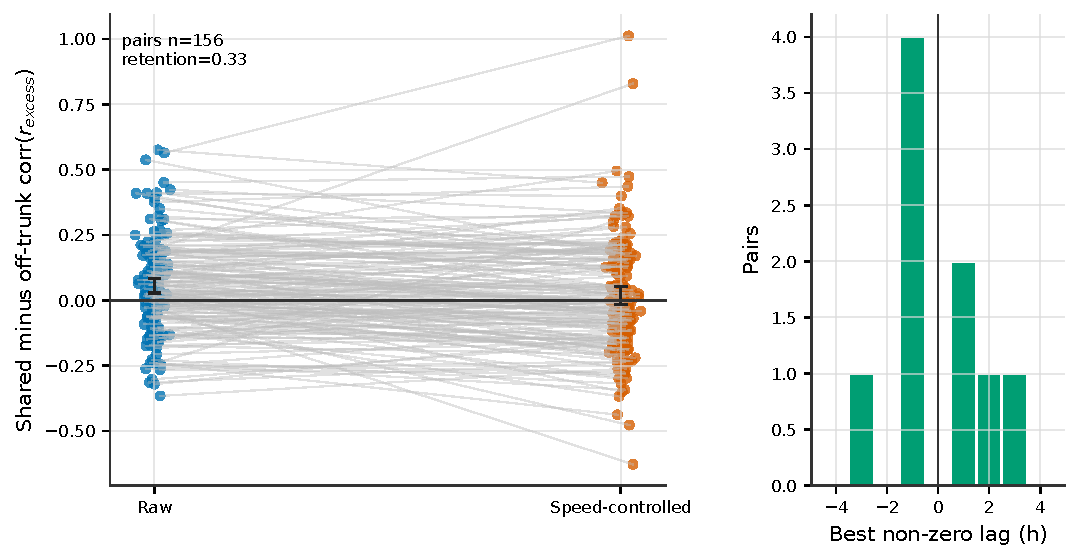
\includegraphics[width=\textwidth]{p4_1_corridor_speed_gate.pdf}
\caption{Shared-trunk co-synchronization before and after controlling the common road state.
Pair-level shared-minus-off-trunk correlations of segment-local corrected synchronization, raw
and after residualizing both line series on the shared-segment mean bus speed; the inset shows
the distribution of significant non-zero lags. Controlling segment speed removes about
two-thirds of the gap and the remainder spans zero, while lead--lag structure is absent.}
\label{fig:corridor}
\end{figure*}

\begin{figure}[t]
\centering
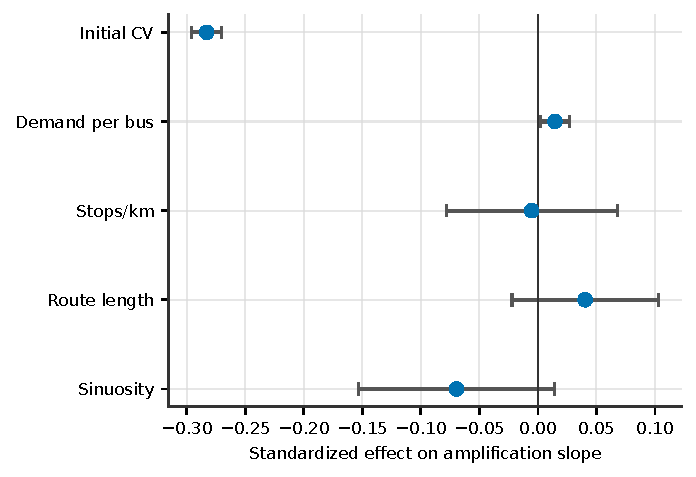
\includegraphics[width=\linewidth]{p4_3_amplification_drivers.pdf}
\caption{Inherited upstream irregularity, not realized load, is the strongest predictor of
downstream headway-CV growth. Standardized effects from a line--direction random-intercept model
with 95\% CIs; the negative upstream-irregularity coefficient is a ceiling effect.}
\label{fig:drivers}
\end{figure}

\section{Robustness: where the oscillators sit}\label{sec:position}

The strongest robustness check in this document concerns something the two-page abstract could
not have surfaced: the spatial distribution of the oscillators themselves.

\subsection{Half the fleet is at a terminal}

Half of all active bus-hours --- 51.1\% --- sit within 10\% of a route terminal, and 27.1\% sit
within 2\% of one (Fig.~\ref{fig:pos}a). This is \emph{after} the layover exclusion described in
Sec.~\ref{sec:data}, which removed 3{,}920 bus-hours. It is not a map-matching artefact:
matching residuals are the same in all three zones (4.13, 3.89, 4.24\,m), and the median
terminal-zone bus-hour spends a third of its time within 5\% of a route end. These are real
vehicles queued for dispatch or turning around.

This matters because buses at a terminal have nearly identical phase by construction --- a
terminal is one place. Computing the order parameter separately within each zone
(Table~\ref{tab:zones}), the terminal zone gives $r_{\rm exc} = 0.997$, essentially perfect
``synchronization'' that encodes only the geometry of dispatch, while the route interior gives
$r_{\rm exc} = -0.187$: in-service buses are \emph{more evenly spread than random}, closer to
the splay state, which is what a functioning dispatch system should look like and what
\cite{chew19} predicts for a stable anti-bunched configuration.

\begin{table}[t]
\centering
\caption{\bf Corrected synchronization by route zone$^{a}$}
\small
\setlength{\tabcolsep}{3.2pt}
\begin{tabular}{lrccrl}
\toprule
Zone & Cells & $r_1$ & $r_{\rm exc}$ & Load & $p$ \\
\midrule
Terminal ($<$2\%)   & 5031 & $0.999$ & $+0.997$ & $+0.000$ & $0.55$ \\
Near (2--10\%)      & 3924 & $0.965$ & $+0.922$ & $-0.000$ & $0.94$ \\
Interior (10--90\%) & 7740 & $0.416$ & $-0.187$ & $-0.003$ & $0.76$ \\
\midrule
Whole route        & 10135 & $0.499$ & $+0.156$ & $+0.035$ & $0.009$ \\
\bottomrule
\end{tabular}
\label{tab:zones}

\smallskip
$^{a}$``Load'' is the standardized coefficient of $\lambda$ on $r_{\rm exc}$ from an OLS model
with line-direction fixed effects and $\log N$, standard errors clustered by line-direction.
The interior 95\% CI is $[-0.025,+0.019]$, excluding the whole-route value.
\end{table}

\subsection{What this does to Result 2}

The whole-route order parameter is a mixture of two regimes with opposite signs, and its value
is governed by the mixing weight. The standardized load effect on $r_{\rm exc}$ is $+0.035$
$([+0.009, +0.061]$, $p = 0.009)$ on the whole route --- close to the $+0.039$ of the accepted
abstract --- but it is statistically indistinguishable from zero in \emph{every} zone taken
separately, including the interior ($-0.003$, $[-0.025, +0.019]$), whose confidence interval
excludes the whole-route value (Fig.~\ref{fig:pos}d). Controlling the cell's terminal fraction
directly attenuates the whole-route effect by 45\%, from $+0.035$ to $+0.019$, and the terminal
fraction itself carries a coefficient of $+1.23$ ($p \approx 10^{-159}$) on $r_{\rm exc}$.

Trimming the route ends confirms the picture (Fig.~\ref{fig:pos}c). Removing 2\% from each end
turns the mean corrected order parameter from $+0.154$ to $-0.121$; at 5\% it reaches $-0.224$.
The correlation between load and corrected synchronization falls from $+0.067$ to $+0.003$ at
5\% trim and $-0.017$ at 10\%. Values rise again at 15--20\% trim, where median $N$ has fallen to
3 and genuine route is being discarded, so the informative range is 2--10\%.

Finally, the scaling collapse of Sec.~\ref{sec:crossover} does not survive either. Repeating the
identical procedure on interior-only cells, the improvement ratio is $1.92$ against a null median
of $2.46$: permutation $p = 0.82$ (Fig.~\ref{fig:collapse}b,c). The apparent scaling belongs to
the terminal--interior mixture, not to the in-service dynamics.

\subsection{How to read this}

We regard this as a refinement of Result 2 rather than its removal, and it points the same way
as the rest of the paper. The demand--synchronization association is real as a description of
the whole-route observable, and it is substantially compositional in origin: higher load goes
with a different terminal/interior mix, and the terminal component is trivially clustered. The
conclusion that there is no critical transition is \emph{strengthened}, because the one scaling
signature that passed on the whole route is compositional too. And the paper's organising claim
--- that what reads as collective synchronization is a mixture of correctable artefacts --- gains
a fourth item on its list, of the same kind as the first three.

The practical lesson generalises beyond this dataset: on an open route, the phase variable is not
equidistributed even under ideal operation, because vehicles accumulate where the route is cut.
Correcting for $N$ while leaving that untouched produces a statistic that measures, to a
substantial degree, how many buses are currently at a terminal. Route position should be a
first-class variable in any field measurement of transit synchronization, and every order
parameter should be reported with its trim setting.

\paragraph{Caveat.} Trimming changes $N$ as well as the phase distribution --- median $N$ falls
from 6 to 3--4 --- so zone-restricted and whole-route numbers are different estimands rather
than a like-for-like comparison, and we report $N$ with every value. That caveat does not
explain the magnitude of the sign change, nor the absence of a load effect in all three zones
separately.

\begin{figure*}[t]
\centering
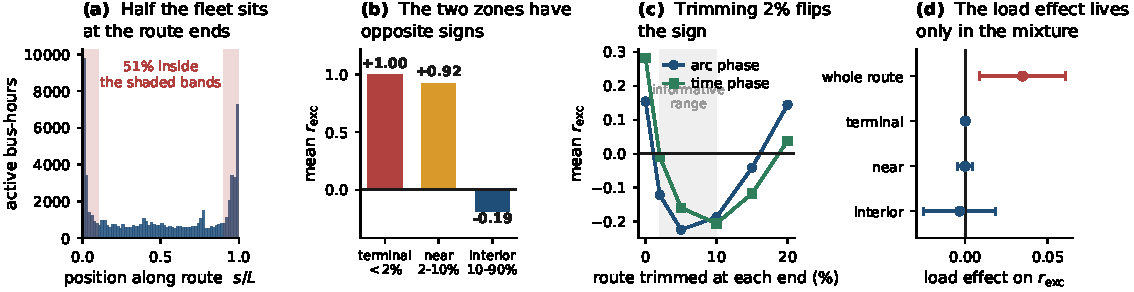
\includegraphics[width=\textwidth]{f2_route_position.pdf}
\caption{Route position governs the whole-route result.
(a) Distribution of bus position along the route: 51\% of active bus-hours lie in the shaded
terminal bands, after layover exclusion. (b) Corrected order parameter within each zone.
Terminal buses are clustered by construction ($r_{\rm exc} = 0.997$); interior buses are more
evenly spread than chance ($-0.187$). (c) Mean corrected order parameter against how much of
each route end is trimmed, for both phase definitions; 2\% flips the sign. (d) Standardized load
effect with 95\% CI: present on the whole route, absent in every zone separately.}
\label{fig:pos}
\end{figure*}

\section{Discussion}\label{sec:discussion}

\subsection{What the corrections buy}

Three things survive the full set of checks. First, the finite-size correction is mandatory and
its foundation is now exact: the null is Kluyver's, the asymptotic expression in common use is
biased where transit data live, and the correction can be validated against a closed form rather
than assumed. Second, the marginal-versus-conditional distinction is real and general --- because
fleet size mediates almost every operational contrast one might want to draw, marginal and
$N$-conditional comparisons answer different questions and both must be reported. Third,
downstream headway amplification is present at roughly the magnitude Newell--Potts predicts,
though not modulated by load at the cell level.

\subsection{Why no transition should have been expected}

The mean-field Kuramoto model has a critical coupling because it has attractive all-to-all
coupling into a common phase, a fixed ensemble, and a closed topology. A bus route has
unidirectional nearest-neighbour coupling, an ensemble that changes membership hourly, an
absorbing bunched state, and a topology cut open once per cycle. The corresponding model,
Eq.~\eqref{eq:np}, has $|A(\theta)| > 1$ for all $k > 0$: instability without a threshold, whose
rate rises smoothly with load. ``Crossover, not criticality'' is therefore the prediction of the
appropriate theory. Reports of bunching phase transitions in idealized closed-loop models
\cite{nagatani01} are not in conflict with this; they describe a different system, one without
terminal reset, without fluctuating $N$, and evaluated without a finite-size null.

\subsection{Generality}

Nothing in either correction is specific to buses. The finite-size problem arises whenever a
phase-coherence statistic is computed on a small, varying ensemble --- which is why
neurophysiology arrived at PPC independently \cite{vinck10}, and why collective-motion studies
computing polarization on small groups face the same bias. The route-position problem generalises
to any system where the phase coordinate is defined on a domain whose occupancy is non-uniform
under ideal conditions, and where the ensemble accumulates at boundaries. The practical
prescription is: validate the null against a closed form where one exists; prefer an
analytically unbiased estimator; report marginal and conditional contrasts separately; and check
whether the order parameter changes sign when the boundary regions are removed.

\subsection{Operational reading}

For an operator, the results say something usable. In-service buses on these 20 lines are
anti-bunched relative to chance, so the dispatch system is working in the route interior. The
measurable irregularity grows downstream at a rate consistent with Newell--Potts, but which cells
degrade is not predicted by their load --- pointing to dispatch and road-state variability rather
than demand as the operational lever. And the shared-trunk co-synchronization that would motivate
inter-line holding strategies is largely a common road state, so an intervention targeting
inter-line coupling would be aimed at the wrong cause.

\section{Limitations}\label{sec:limits}

The absence of a shared vehicle key between telemetry and ticketing confines demand to
line-hour resolution; $\lambda$ is realized load per active bus, not exogenous demand, and no
vehicle-level dwell mechanism can be tested, which is why the mediation result of
Sec.~\ref{sec:mechanisms} is inconclusive rather than negative. Zone-restricted estimates change
$N$ as well as position and are not like-for-like comparisons with whole-route estimates. The
collapse test has three free parameters and five strata, so even its whole-route success is weak
evidence considered alone; we rely on the permutation control rather than on goodness of fit.
Our null models assume exchangeability of phases within a cell, which the unidirectional
coupling structure formally violates. Speed control in the corridor analysis may absorb part of a
genuine coupling channel as well as the common shock. Finally, this is nineteen days in one city,
and the terminal geometry of Niter\'oi's network --- with substantial layover space at route ends
--- may be more pronounced than elsewhere; replication on a second network is the natural next
step.

\section{Conclusion}

What appears as collective synchronization in raw transit data can be a mixture of finite-size
bias, route-position structure, operational dispatch irregularity, and common road-state shocks.
In Niter\'oi, once the order parameter is corrected against its same-$N$ random baseline, the
demand dependence is a smooth crossover rather than a critical transition; downstream
amplification tracks inherited irregularity more than realized load; and shared-corridor
co-synchronization is largely a shared road state. The extended analysis in this document
sharpens two of those statements. The weekend effect is abolished rather than reversed once
conditioned on fleet size, in every estimator and null we tried. And the demand association on
the whole route is substantially a terminal/interior mixture: in the route interior, where the
Newell--Potts mechanism can actually operate, buses are more evenly spread than chance. Meanwhile
the appropriate model predicts instability without a threshold, so the smooth load dependence
reported across this literature is what theory expects rather than a weakened version of a
transition.

The methodological point is not about buses. Any field measurement of synchronization on a
finite, fluctuating ensemble faces the first correction, and any measurement whose phase
coordinate lives on a bounded domain faces the second. Neurophysiology reached the same
conclusion independently and answered it with the pairwise phase consistency \cite{vinck10};
studies of collective motion computing polarization or alignment on small flocks, schools or
cell groups have the identical $1/\sqrt{N}$ floor; and the same applies to phase-locking indices
in coupled laser arrays, Josephson junction arrays, and circadian ensembles measured cell by
cell, wherever the number of contributing units is small and varies with the condition being
compared. The prescription that transfers is four lines long: validate the null against a closed
form where one exists rather than an asymptotic expression; prefer an estimator that is unbiased
under the alternative and not only under the null; report marginal and conditional contrasts as
separate estimands whenever ensemble size mediates the comparison; and check whether the order
parameter changes sign when the boundary regions of the domain are removed. Applied here, those
four steps turned an apparent demand-driven synchronization transition into a mixture of
correctable artefacts. Two steps would sharpen identification further within transit: a
propagation-aware coupling model able to separate inter-line transfer from shared road shocks,
and vehicle-linked boarding data with a cleaner dwell signal to test the demand mechanism
directly.

\appendix

\section{Reproducibility}\label{app:repro}

All analysis is implemented in a small library (\texttt{src/netmob/}: \texttt{theory},
\texttt{nulls}, \texttt{estimators}, \texttt{phase}, \texttt{stats}) driven by scripts in
\texttt{pipelines/}, with fixed seeds throughout. Rebuilding every number in this report from the
released dataset requires, in order: \texttt{build\_cells.py}, \texttt{sweep.py},
\texttt{terminal\_sensitivity.py}, \texttt{theory\_tests.py}, \texttt{route\_position.py} and
\texttt{figures.py}. A standalone script, \texttt{verify\_vehicle\_join.py}, re-derives the
zero-overlap result of Sec.~\ref{sec:data} directly from the released CSVs in one command,
because that single fact fixes the identification scope of everything else.

Twenty-one unit tests (\texttt{tests/test\_theory.py}) execute the validations the argument
depends on, so that the claims are checkable rather than asserted: the Monte Carlo null against
Kluyver's exact CDF for $N = 2\ldots8$; $\mathbb{E}[r_1^2] = 1/N$ to within 2\% for
$N = 2\ldots12$; $\mathbb{E}[r_1] = 2/\pi$ at $N=2$; the PPC identity against its pairwise
definition; that PPC and $r_{\rm exc}$ have null expectation zero at every $N$ while the PIT is
exactly standard normal; that $r_2$ detects two antipodal clusters invisible to $r_1$; and the
Newell--Potts results of Sec.~\ref{sec:assump}, including that $|A(0)| = 1$ exactly, that
$\theta = \pi$ maximises growth at $1+2k$, that headway deviations on a ring conserve cycle time,
and that the mode-1 growth rate matches Eq.~\eqref{eq:mode1growth}.

As a consistency check on the refactored pipeline, aggregating the per-bus phase table back to
cell level reproduces the order parameters of the original four-phase analysis to
$3.3\times10^{-16}$ across all 11{,}641 cells, with identical $N$. Differences between this
document and the accepted abstract therefore come from method, not from divergent data handling.

\section{Where the abstract reviews are addressed}\label{app:reviews}

For convenience, the points raised on the two-page abstract and the sections that take them up.

\begin{itemize}\itemsep2pt
\item \emph{The dwell-mediation null could be misread as evidence against the mechanism; a
      caveat at the first mention of the data would help.} The limitation is now stated where
      the missing vehicle key is introduced (Sec.~\ref{sec:data}), before any result depends on
      it, and repeated at the result itself (Sec.~\ref{sec:mechanisms}) and in
      Sec.~\ref{sec:limits}.
\item \emph{The methodological contribution should come earlier.} The Introduction now opens by
      stating that this is a study of a measurement problem before it is a study of buses; its
      second paragraph makes the observable, not the transit application, the central claim; and
      the itemised list that follows separates the six methodological additions from the
      empirical ones.
\item \emph{The mathematical motivation for the finite-size correction should be developed, and
      the choice of normalisation justified.} Sec.~\ref{sec:null} derives the bias from
      Kluyver's exact solution of Pearson's random walk with exact moments, and shows the
      Rayleigh asymptotic in common use is biased where these data live.
      Sec.~\ref{sec:criterion} states five explicit criteria for judging a normalisation and
      evaluates all five estimators against them --- concluding that the abstract's choice is
      not optimal on three of the five, and recommending PPC instead.
\item \emph{Compare against alternative normalisation strategies or existing measures that
      mitigate finite-size effects.} Sec.~\ref{sec:estimators} and Table~\ref{tab:gradient}
      compare five, including the pairwise phase consistency developed in neurophysiology for
      the same problem \cite{vinck10} and the classical Rayleigh statistic.
\item \emph{The dependence on the null model and the assumptions behind the random-phase
      simulations deserve explicit discussion.} Sec.~\ref{sec:nullmodels} builds four nulls
      spanning a nested hierarchy of preserved structure, separates the three assumptions
      embedded in the null and states how each fails here, and reports every headline result
      under all four.
\item \emph{The conclusion should emphasise applicability beyond urban transportation.} The
      closing paragraph names the domains where the same two corrections apply and reduces the
      prescription to four transferable steps; Sec.~\ref{sec:discussion} develops the argument.
\end{itemize}

\begin{thebibliography}{99}

\bibitem{newell64} G.~F. Newell and R.~B. Potts, ``Maintaining a bus schedule,'' in
\emph{Proc. 2nd Conf. Australian Road Research Board}, Melbourne, vol.~2 (1964), pp. 388--393.

\bibitem{saw19} V.-L. Saw, N.~N. Chung, W.~L. Quek, Y.~E.~I. Pang, and L.~Y. Chew,
``Bus bunching as a synchronisation phenomenon,'' Sci. Rep. \textbf{9}, 6887 (2019).

\bibitem{strogatz00} S.~H. Strogatz, ``From Kuramoto to Crawford: exploring the onset of
synchronization in populations of coupled oscillators,'' Physica D \textbf{143}, 1--20 (2000).

\bibitem{kuramoto75} Y.~Kuramoto, in \emph{Int. Symp. Math. Problems in Theor. Phys.},
Lect. Notes Phys. \textbf{39} (1975), p.~420.

\bibitem{schlapfer21} M.~Schl\"apfer, L.~Dong, K.~O'Keeffe, \emph{et al.},
``The universal visitation law of human mobility,'' Nature \textbf{593}, 522--527 (2021).

\bibitem{netmob26} F.~Domingos, H.~T. Marques-Neto, B.~Pereira, \emph{et al.},
arXiv:2605.20263 (2026).

\bibitem{kluyver05} J.~C. Kluyver, ``A local probability problem,'' Proc. Sect. Sci.
Koninklijke Akademie van Wetenschappen te Amsterdam \textbf{8}, 341--350 (1905).

\bibitem{vinck10} M.~Vinck, M.~van Wingerden, T.~Womelsdorf, P.~Fries, and C.~M.~A. Pennartz,
``The pairwise phase consistency: a bias-free measure of rhythmic neuronal synchronization,''
NeuroImage \textbf{51}, 112--122 (2010).

\bibitem{daido90} H.~Daido, ``Intrinsic fluctuations and a phase transition in a class of large
populations of interacting oscillators,'' J. Stat. Phys. \textbf{60}, 753--800 (1990).

\bibitem{chew19} L.~Y. Chew, V.-L. Saw, and Y.~E.~I. Pang, ``Stability of anti-bunched buses and
local unidirectional Kuramoto oscillators,'' arXiv:1912.06470 (2019).

\bibitem{gershenson09} C.~Gershenson and L.~A. Pineda, ``Why does public transport not arrive on
time? The pervasiveness of equal headway instability,'' PLoS ONE \textbf{4}, e7292 (2009).

\bibitem{nagatani01} T.~Nagatani, ``Bunching transition in a time-headway model of a bus
route,'' Phys. Rev. E \textbf{63}, 036115 (2001).

\bibitem{hong07} H.~Hong, H.~Chat\'e, H.~Park, and L.-H. Tang, ``Entrainment transition in
populations of random frequency oscillators,'' Phys. Rev. Lett. \textbf{99}, 184101 (2007).

\bibitem{daganzo09} C.~F. Daganzo, ``A headway-based approach to eliminate bus bunching:
systematic analysis and comparisons,'' Transp. Res. B \textbf{43}, 913--921 (2009).

\end{thebibliography}

\end{document}
